%\section{Results}
%\label{sec:Results}
%% Results should be clear and concise.

The experiment to test the hypothesis that participants in a virtual reality (VR) experiment would show a trend towards choosing complex environments over simple ones when given the task of identifying the more comfortable facade design, wa conducted at the Kyushu University campus in Fukuoka, Japan, over a period of 15 days, from October 12 to 30, 2023, during the work hours between 10:00 and 18:00.

A total of 10 participants took part in the experiment, primarily consisting of university students and faculty members.
The participants had diverse professional backgrounds, as shown in Figure \ref{fig:ParticipantBackgroundChart}, with over \(67\%\) being students from various faculties, approximately \(33\%\) having a construction background, and \(14\%\) reporting previous experience in facade design, as indicated in Figure \ref{fig:YearsExperienceChart}

%% Participant background chart and years of experience
    \begin{table*}[htb]
        \centering
        \small
        \begin{tabularx}{\textwidth}{X X}
            \centering
            % trim=left 0 down 50 right 0 top 50
            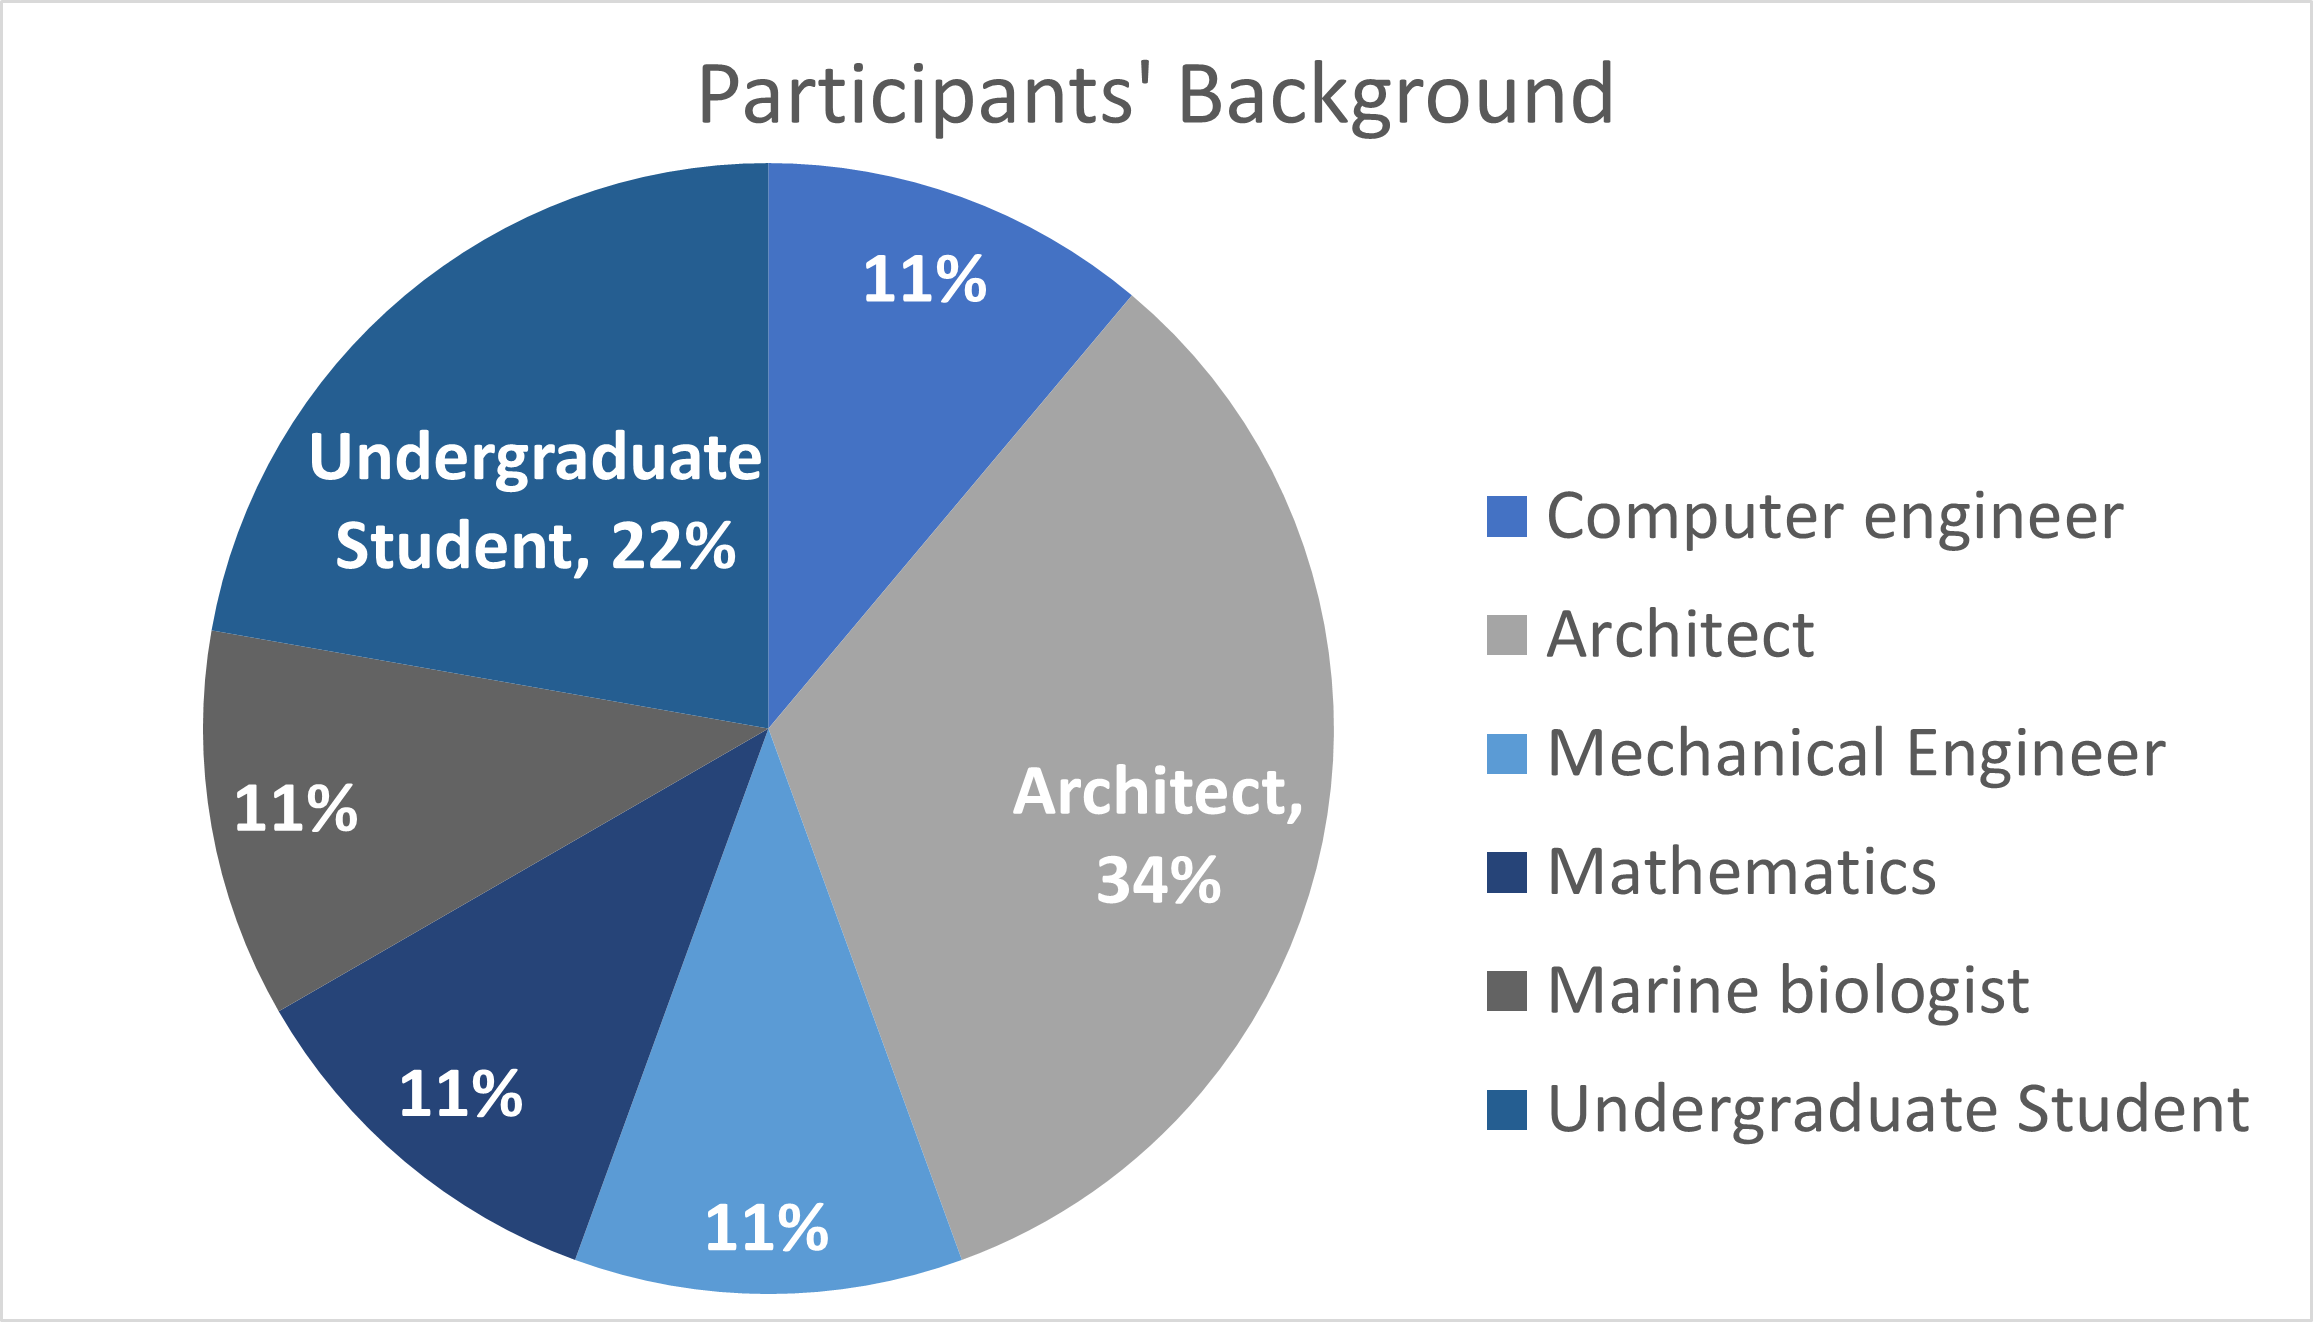
\includegraphics[width=\linewidth, trim=0 60 0 0]{Images/SurveyBackground}
            \captionof{figure}{This chart shows the professional backgrounds of participants involved in the facade design complexity analysis experiment.}
            \label{fig:SurveyBackgroundChart} &
            \centering
            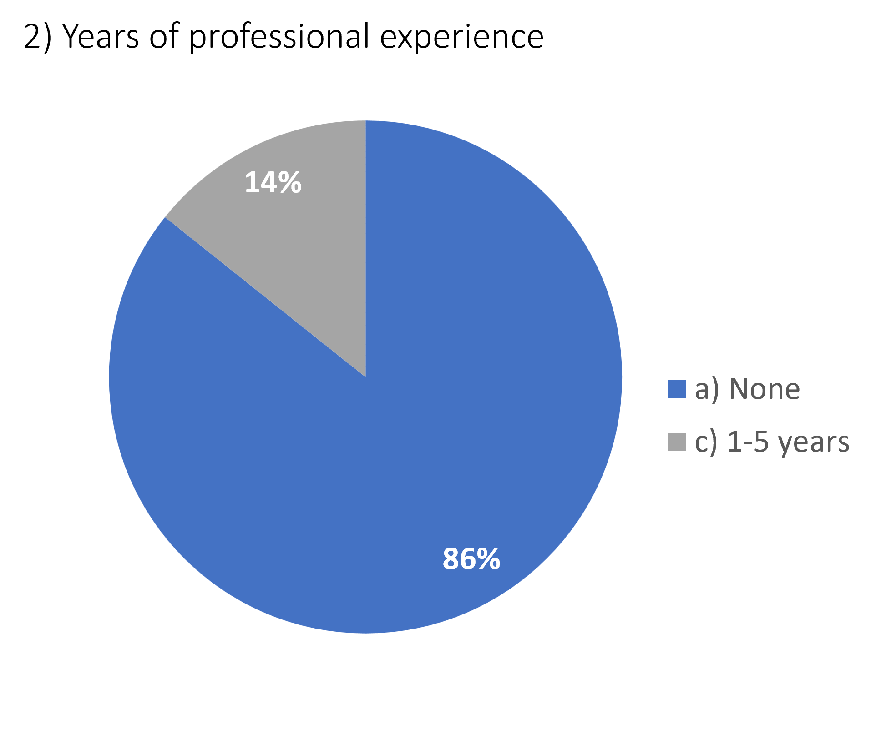
\includegraphics[width=\linewidth, trim=0 60 0 0]{Images/SurveyExperience}
            \captionof{figure}{This chart displays the experience levels in facade design of participants for the study complexity analysis in building design.}
            \label{fig:SurveyYearsExperienceChart}
        \end{tabularx}
    \end{table*}

Regarding the first theme of analysis addressed during the `VR Interaction' stage, related to user tolerance to complex facade design, all participants completed the facade selection task for all three patterns, resulting in a total of 30 experiment sessions.
For each pattern, one answer was recorded based on the facade variation, labeled by the level of complexity, that the participant choose as the most comfortable.

%!Complexity level chosen bar chart
These outcomes were summarized in a bar chart referred to as `Complexity level Chosen graph' as depicted in Figure \ref{fig:ComplexityLevelChosenChart}.

    % Complexity level chosen Chart
    \begin{figure}[htb]
        \centering
        %trim=100 180 100 120, clip
        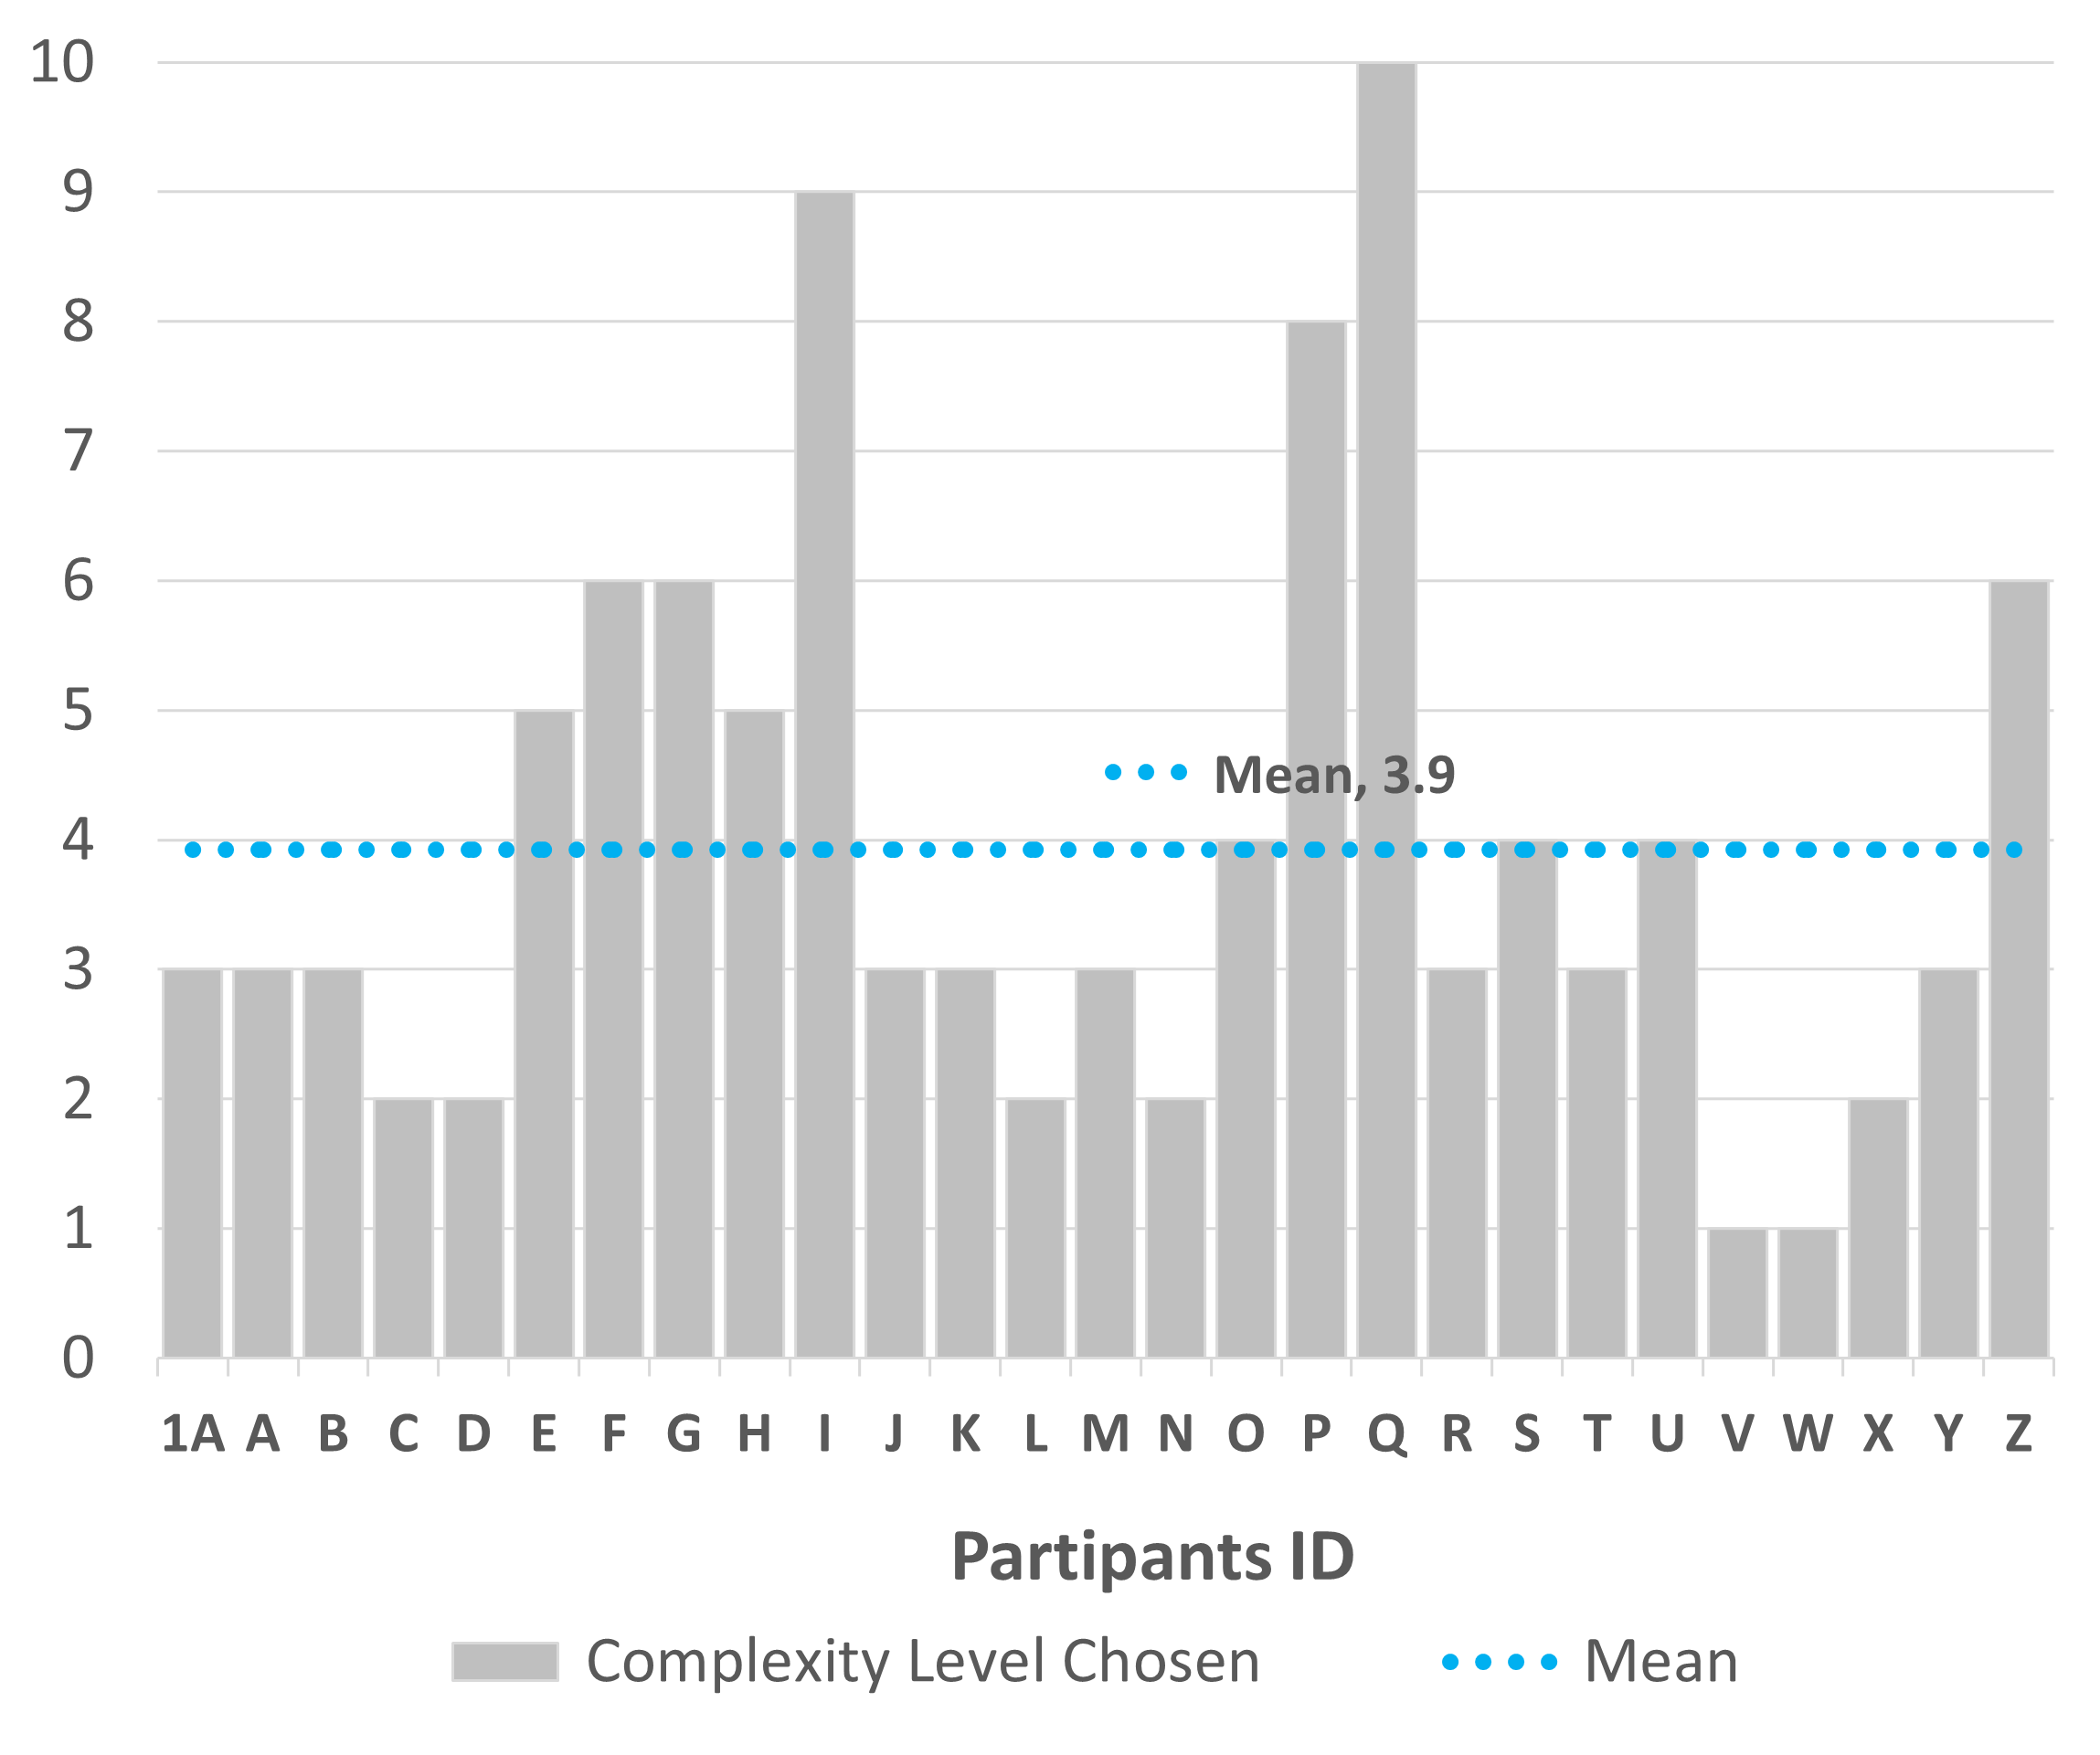
\includegraphics[width=\linewidth]{Images/ComplexityLevelChosenChart}
        \caption{Chart displaying participants' preferred complexity levels among the ten options during the VR simulation stage of the experiment for all three patterns.}
        \label{fig:ComplexityLevelChosenChart}
    \end{figure}

The Complexity chosen level results, depicted in the `Complexity level Chosen graph' in Figure \ref{fig:ComplexityLevelChosenChart}, showcased a diverse range of preferences among the 30 experiment sessions, with most of them allocated bellow the `level 5' of complexity and only five instances going above this line, returning overall an average of  complexity level \(3.9\) as the preferred one among the 10 levels defined for the facade variations for all three patterns.

The preferred complexity level depicted on this graph exhibited a wide distribution, as indicated by the current standard deviation of \(2.3\).

%!Complexity level chosen probability graph

The probability bell graph displayed in Figure \ref{fig:ProbabilityComplexitylevelChart} further illustrates the distribution of choices in the results, emphasizing that there is a \(40\%\) probability of a focus group selecting and answer close to the level 4 of complexity as defined by the facade variations with a standard deviation of \(11\%\)in predicting individual data points or outcomes.

     % Probability Chart and Complexity level per Pattern
    \begin{table*}[htb]
        \centering
        \small
        \begin{tabularx}{\textwidth}{X X}
            \centering
            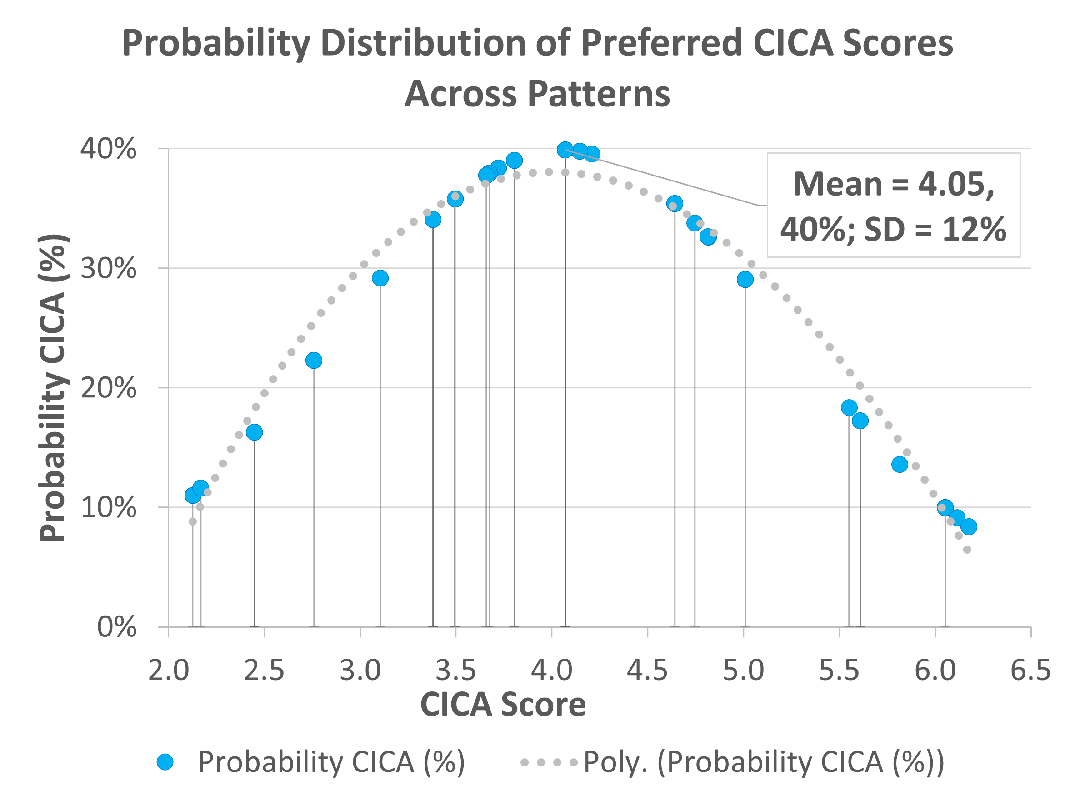
\includegraphics[width=\linewidth, trim=0 0 0 20]{Images/ProbabilityPreferredComplexitylevel}
            \captionof{figure}{Scatter graph illustrating the probability distribution of preferred complexity levels for facade design across all three patterns, derived from data collected during the VR stage of the experiment.}
            \label{fig:ProbabilityComplexitylevelChart} &
            \centering
            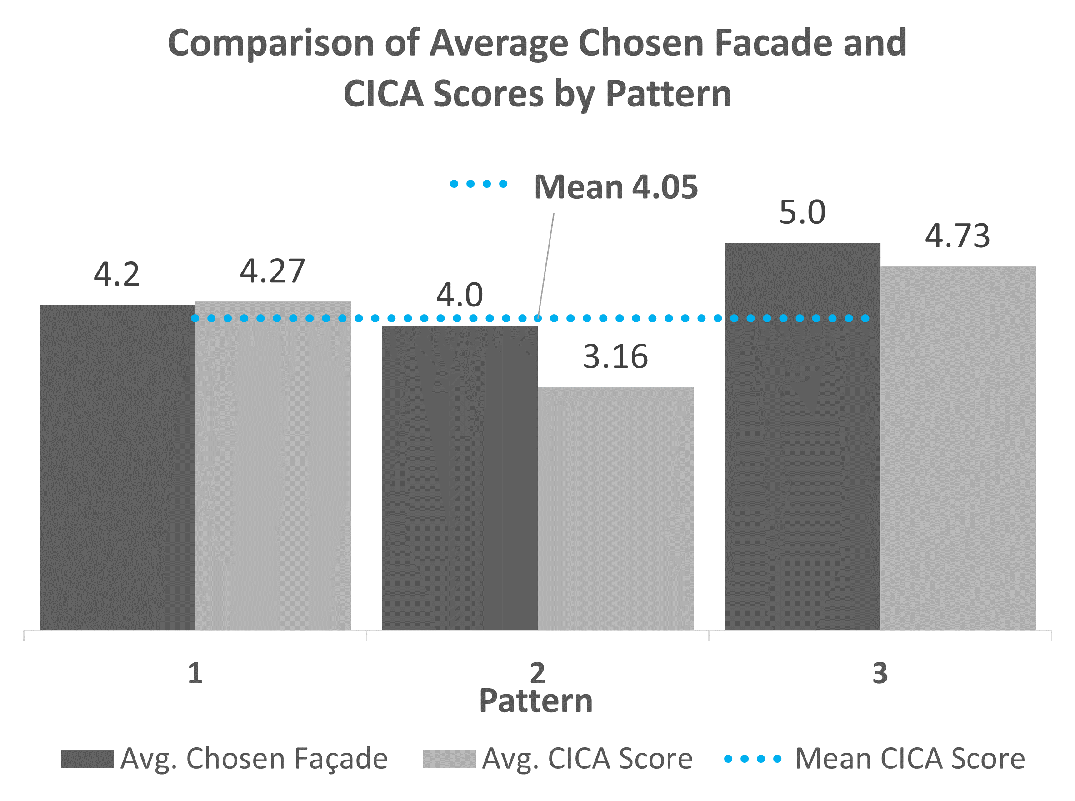
\includegraphics[width=\linewidth, trim=0 0 0 20]{Images/PreferredComplexityLevelPerPattern}
            \captionof{figure}{Average preferred complexity level per pattern by participants during the VR simulation (Overall Mean complexity level = \(4.9\)).}
            \label{fig:ComplexityLevelPerPattern}
        \end{tabularx}
    \end{table*}

%% probability preferred complexity level Chart
%    \begin{figure}[htb]
%        \centering
%        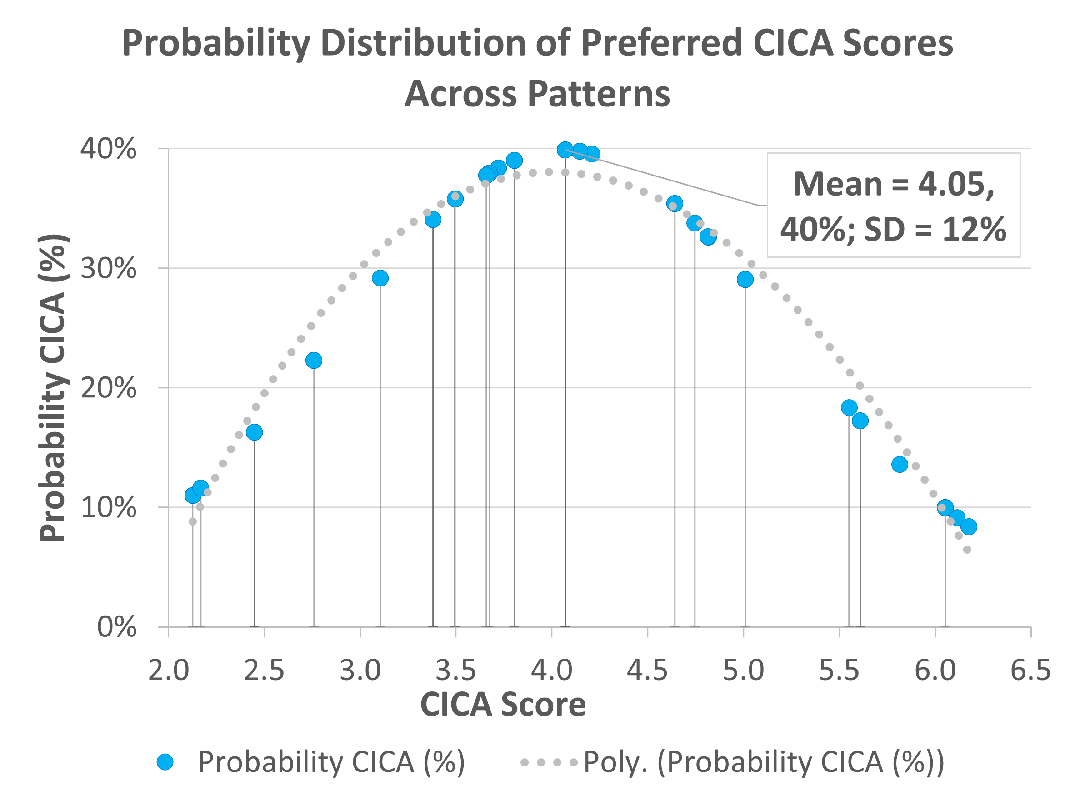
\includegraphics[width=\linewidth]{Images/ProbabilityPreferredComplexitylevel}
%        \caption{Scatter graph illustrating the probability distribution of preferred complexity levels for facade design across all three patterns, derived from data collected during the VR stage of the experiment.}
%        \label{fig:ProbabilityComplexitylevelChart}
%    \end{figure}

%!Complexity level per pattern graph

Analyzing the average complexity level chosen per pattern (Figure \ref{fig:ComplexityLevelPerPattern}) revealed that the average choice across all patterns remains close to the overall average complexity level \(3.9\).

%===============Continue from here for the accuracy section

as radial graphs, referred to as "accuracy analysis graphs," as depicted in Figure \ref{fig:Accuracyscattergraph}.

 %% Figure Accuracy graph
    \begin{figure*}[htb]
      \centering
      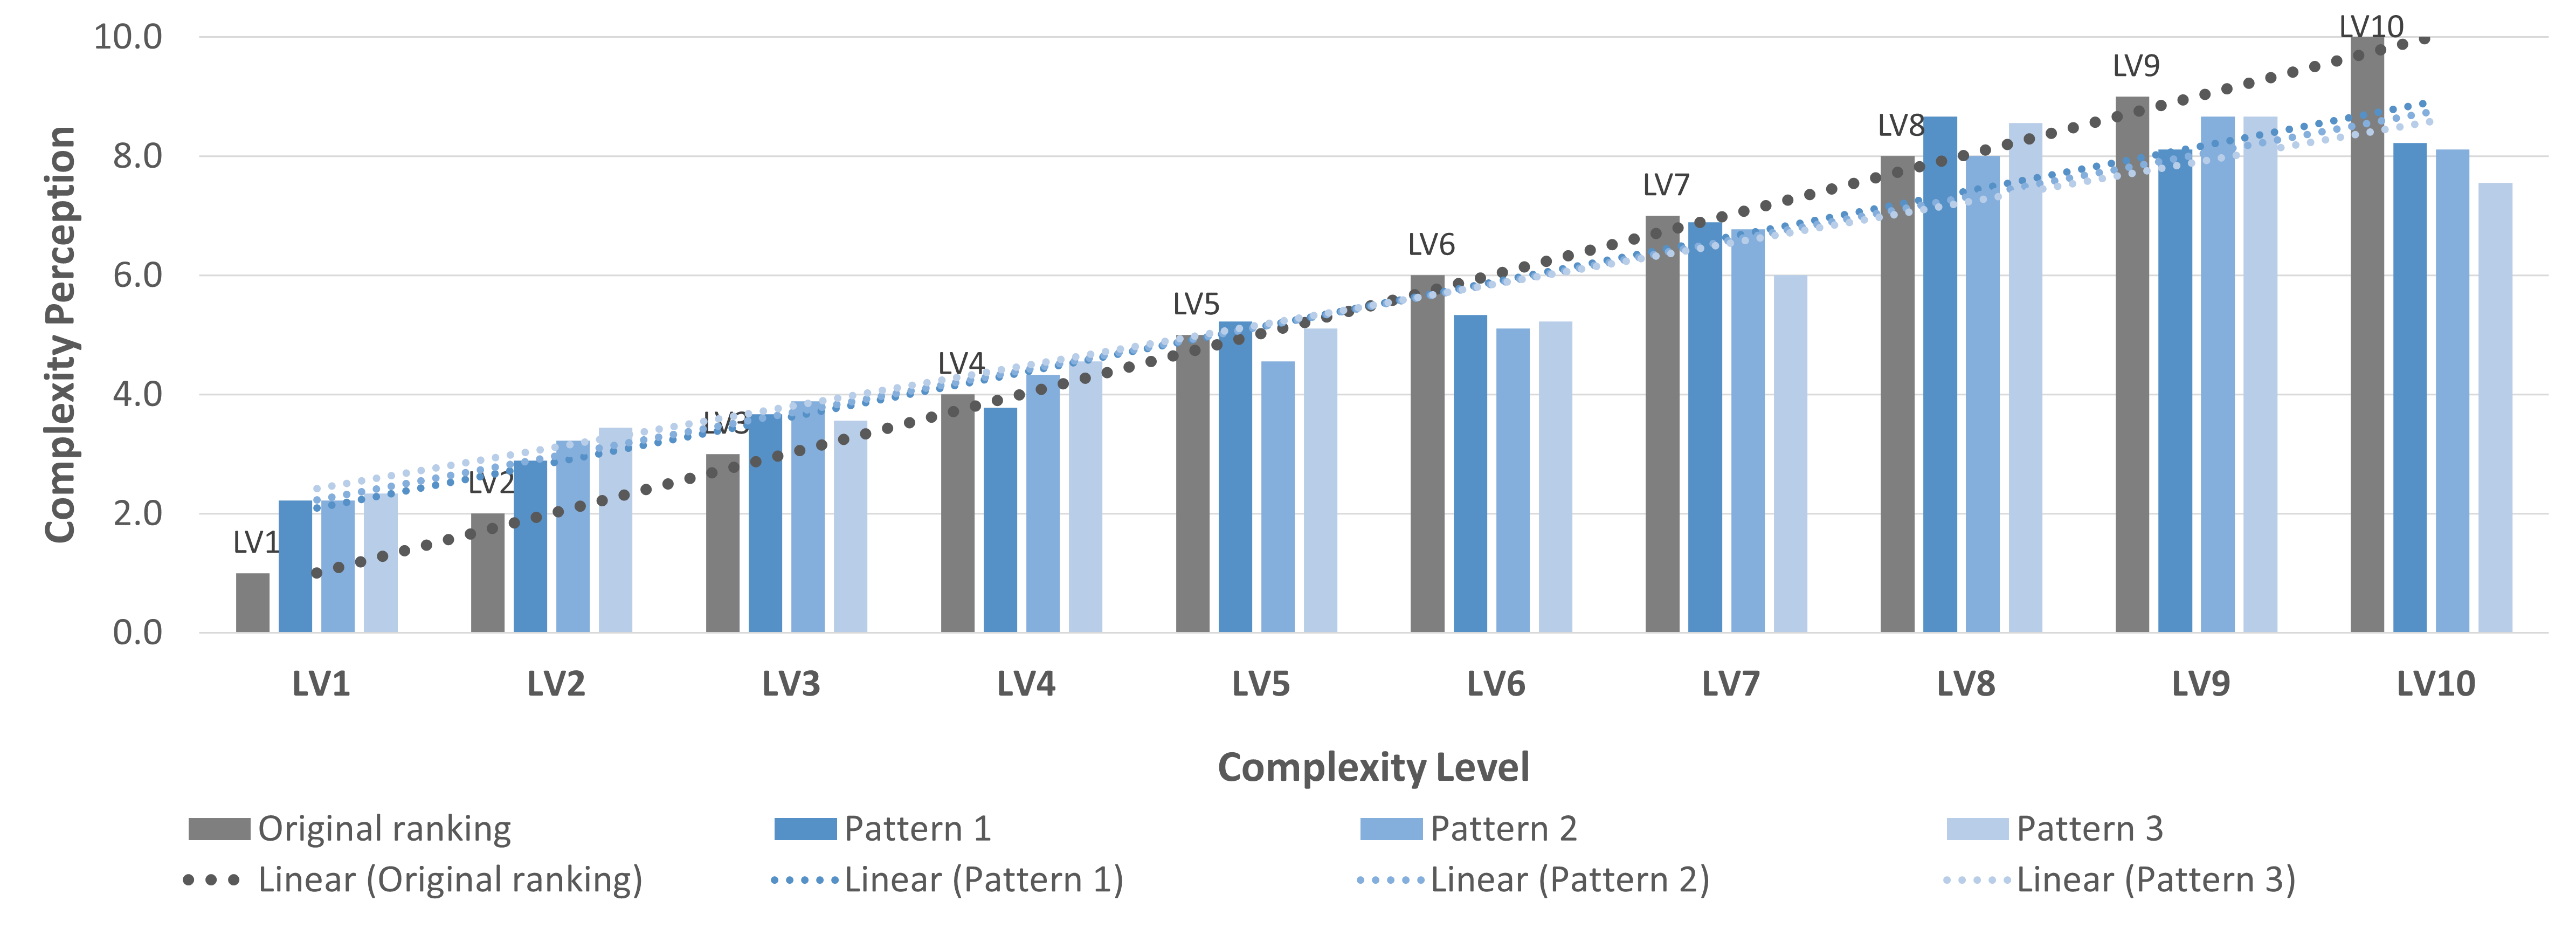
\includegraphics[width= \linewidth, trim=0 0 0 0]{Images/ComplexityPerceptionPerLevel}
      \caption{This graph highlights participants' perception of complexity for the 10 variations within three patterns in contrast to the original ranking. It visually represents the differences between participants' perceived complexity and the initial rankings during the screen-based complexity assessment stage of the experiment.}
      \label{fig:ComplexityPerceptionPerLevel}
    \end{figure*}

In these graphs, the center serves as a reference point, representing the top recommendation provided by the optimization system for each specific site.
The coordinates of this center point vary for each site, reflecting the distinct optimal locations suggested by the system.
On the other hand, the participants' chosen locations are plotted on the graph, precisely indicating the positions they deemed most suitable for the new educational building within the boundaries of the site.

The placement of each participant's chosen location on the graph is based on its actual geographical coordinates, ensuring an accurate representation of their decision-making process.
The distance between each participant's chosen location and the center reflects the deviation error from the system's top recommendation, allowing for a clear assessment of how closely participants' choices align with the data-driven optimization results.

Furthermore, the orientation of each chosen location on the graph provides valuable insights into the direction in which participants opted to position the building, allowing for a comprehensive understanding of their decision-making rationale.
Overall, these accuracy analysis graphs present an actual representation of the chosen locations on the physical site, capturing both spatial proximity and directional preferences relative to the system's top recommendation.

The purpose of the analysis was to evaluate the reduction in the deviation error between the preferred SLP location recommended by our Multi-objective optimization (MOO) model and the location ultimately chosen by the experiment participants in both the ``screen-based'' and "VR interaction" stages of the experiment.

By analyzing the accuracy analysis graphs, the contribution of the VR system was determined by examining the vector resultant from the center point (top recommendation) to the participant's chosen location.
A reduction in the vector magnitude in the "VR answer" compared to the "screen-based answer" indicated an improvement percentage, while an increase represented a decline.
This analysis allowed us to quantify the impact of VR immersion on participants' decision-making accuracy in SLP design.

The accuracy analysis results, depicted in the "Accuracy improvement" bar chart in Figure \ref{fig:ImprovementChart}, showcased varying degrees of improvement among the 39 experiment sessions, with only three cases showing a decline.
On average, there was a \(48.3\%\) improvement among the participants.

The accuracy analysis results, illustrated in the "Accuracy improvement" bar chart (Figure \ref{fig:ImprovementChart}), revealed varying degrees of improvement among the 39 experiment sessions, with only three cases showing a decline.
On average, there was a significant \(48.3\%\) improvement among the participants.

    % Complexity perception Chart
    \begin{figure}[htb]
        \centering
        %trim=100 180 100 120, clip
        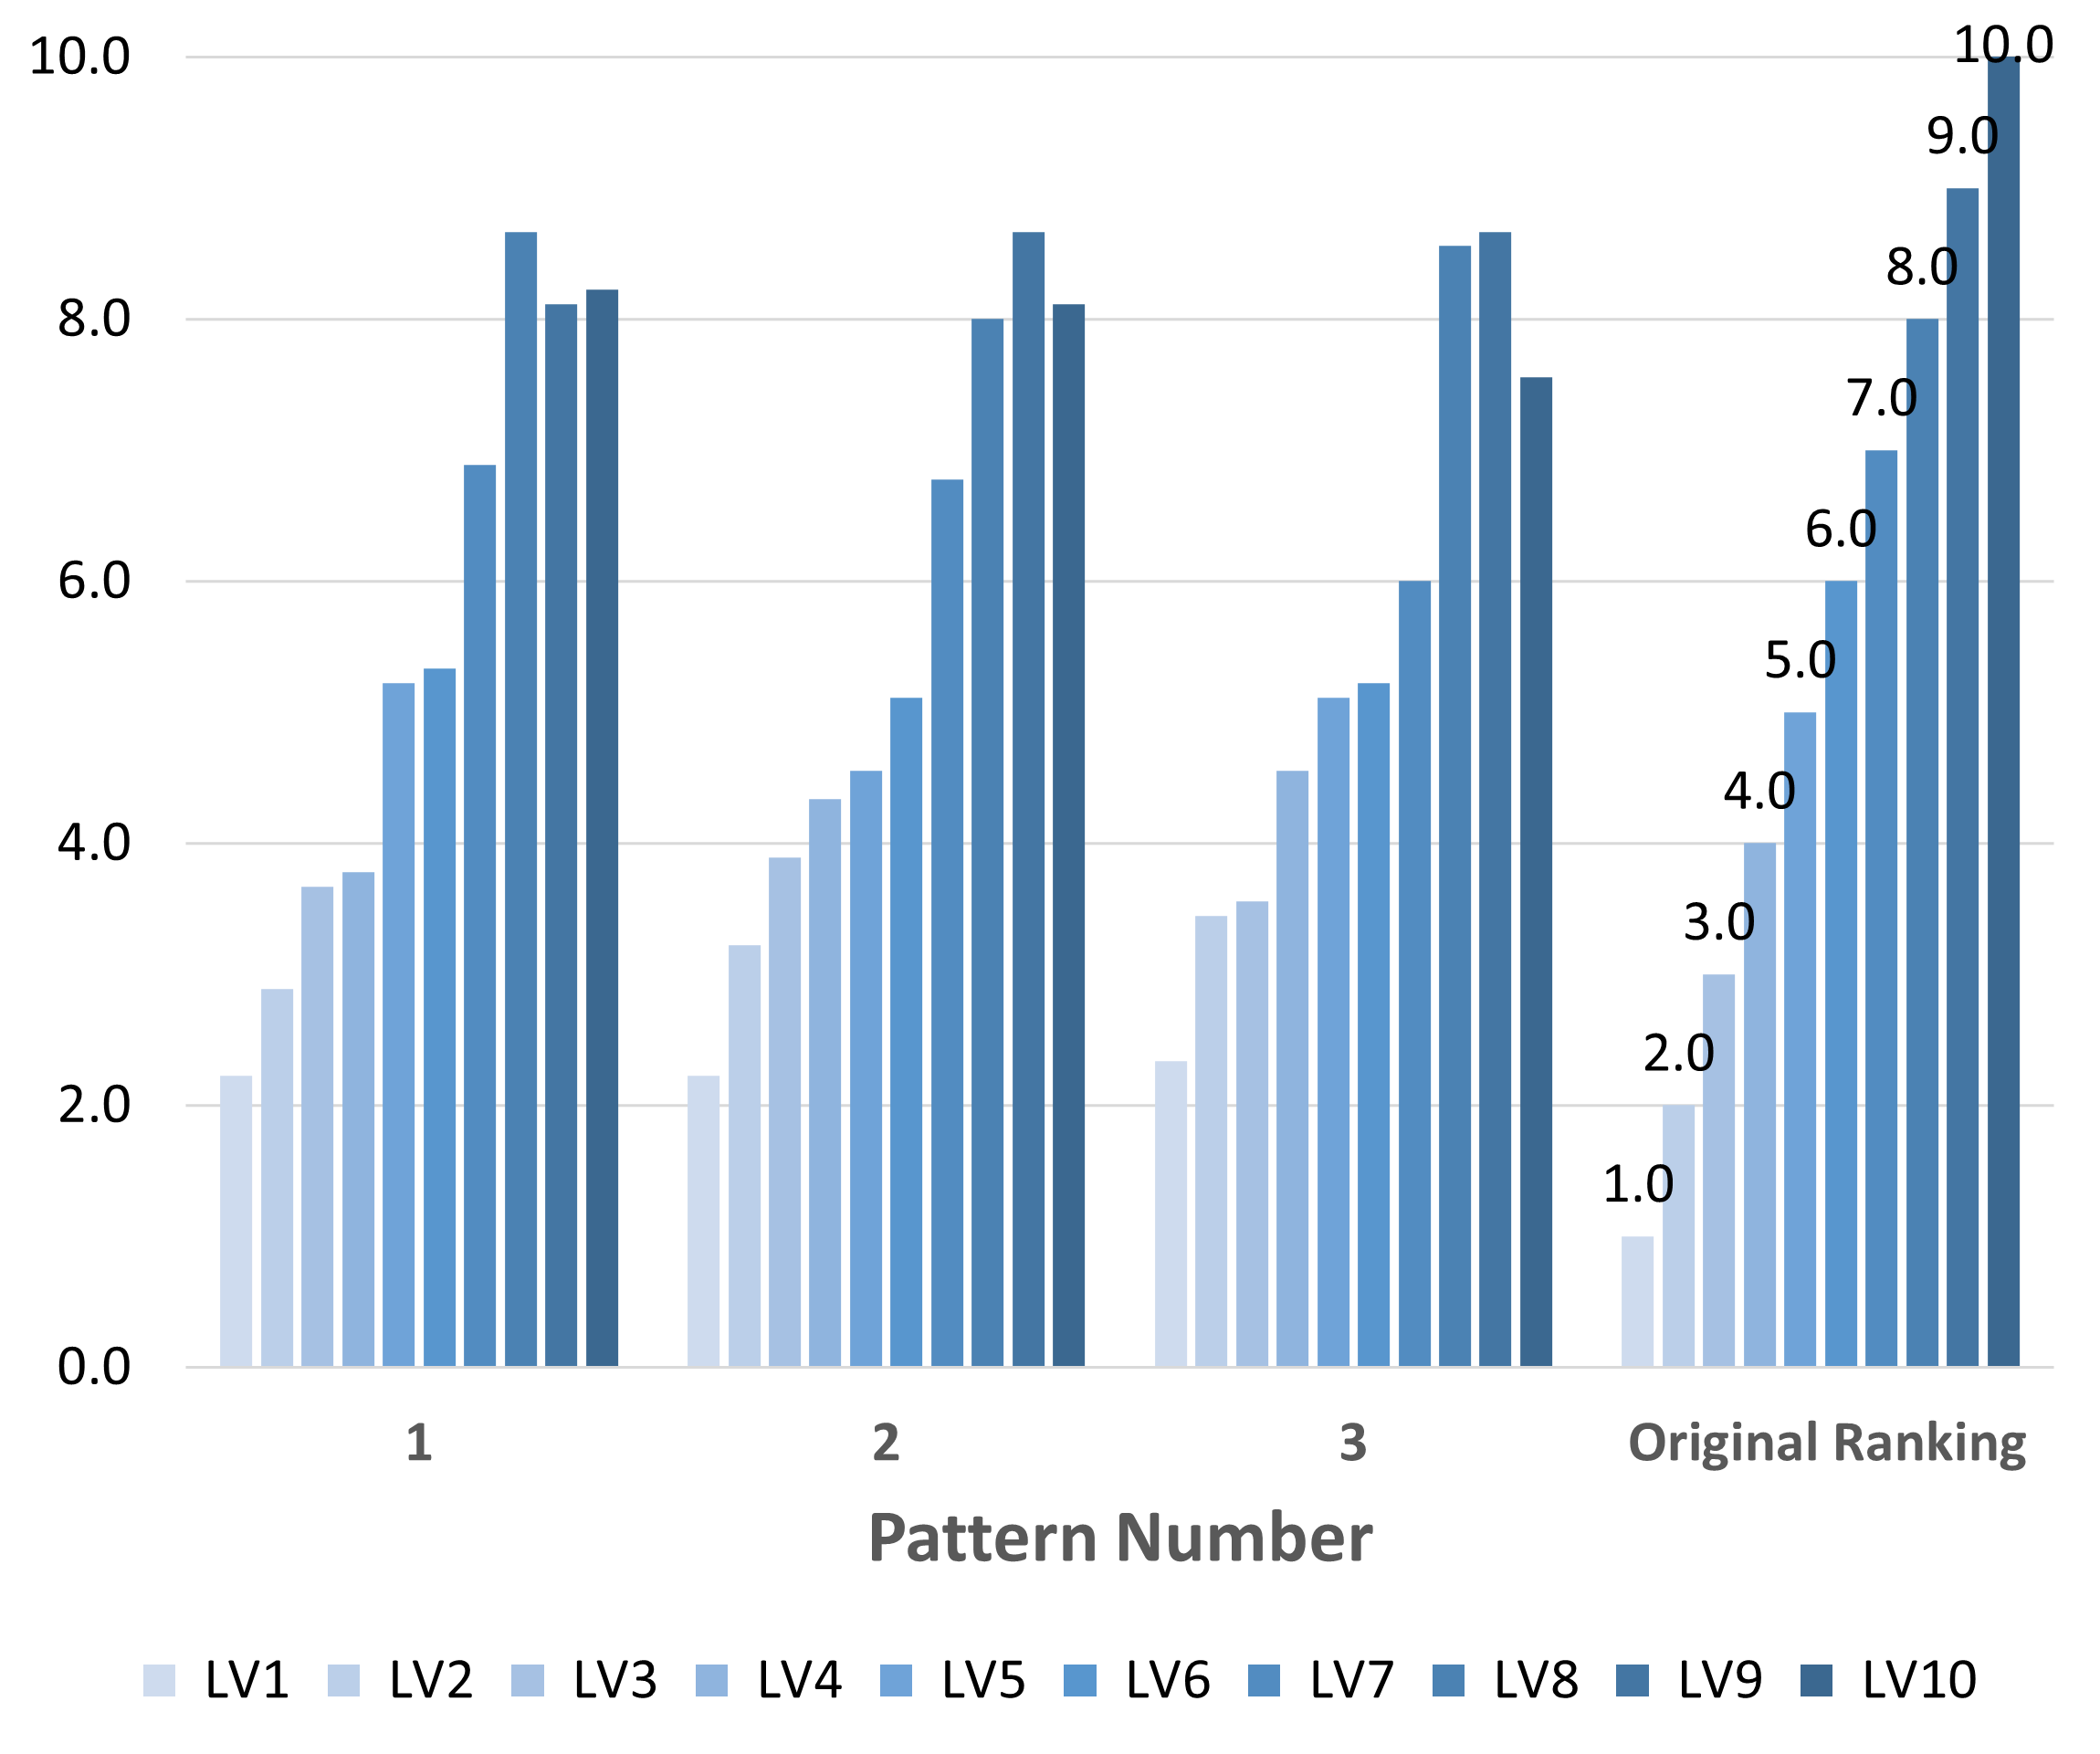
\includegraphics[width=\linewidth]{Images/ComplexityPerceptionChart}
        \caption{Chart depicting participants' complexity perception related to the three patterns. Insights into participants' perception of complexity concerning specific patterns during the screen-based complexity assessment phase of the experiment.}
        \label{fig:ComplexityPerceptionChart}
    \end{figure}

%! Post experiment survey results

The survey results provided additional insights into the influence of VR interaction and data-driven optimization for SLP. The ``influence perception'' section of the survey, depicted in Figure\ref{fig:PerceptionSatisfactionSurveyResults}, indicated that the system scored above 5 on a 7-point Likert scale for all questions, suggesting a positive influence of the VR strategy in introducing data-driven recommendations.
This finding aligned with the accuracy improvement percentage results observed in the accuracy analysis (Figure\ref{fig:ImprovementChart}).


  %% Complexity Perception Survey results
    \begin{table*}[htb]
        \centering
        \small
        \begin{tabularx}{\textwidth}{X X}
            \centering
            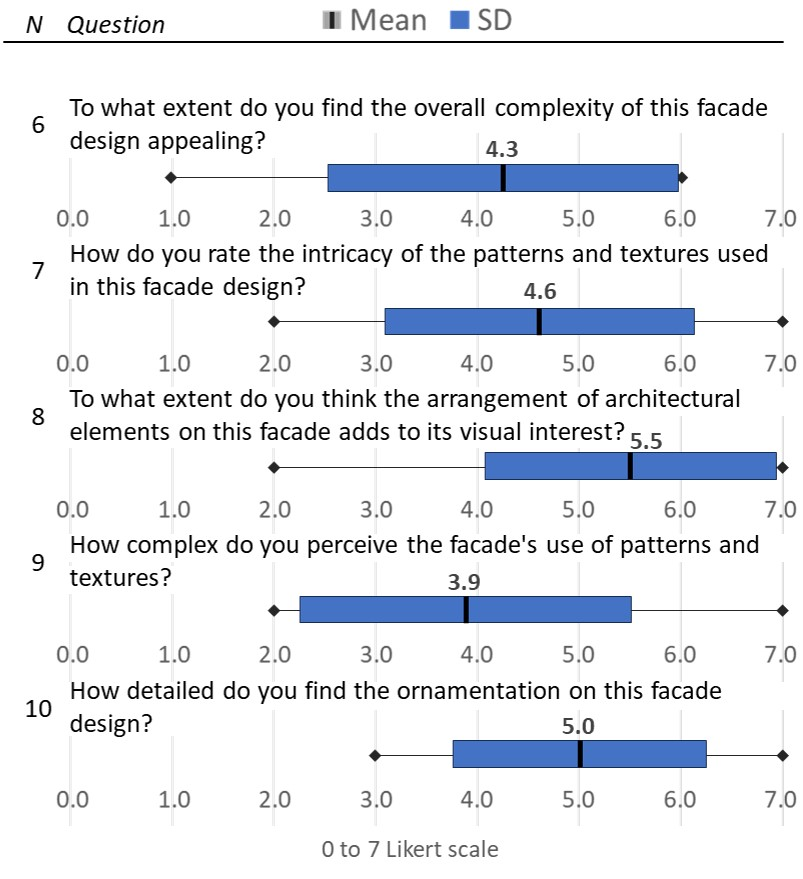
\includegraphics[width=\linewidth]{Images/SurveyPart1Complexity}
            \captionof{figure}{User Satisfaction section questions from User Survey of SLP System. \- (n = 17), 1 - strongly disagree, 7 - strongly agree}
            \label{fig:SurveyQuestions6-10} &
            \centering
            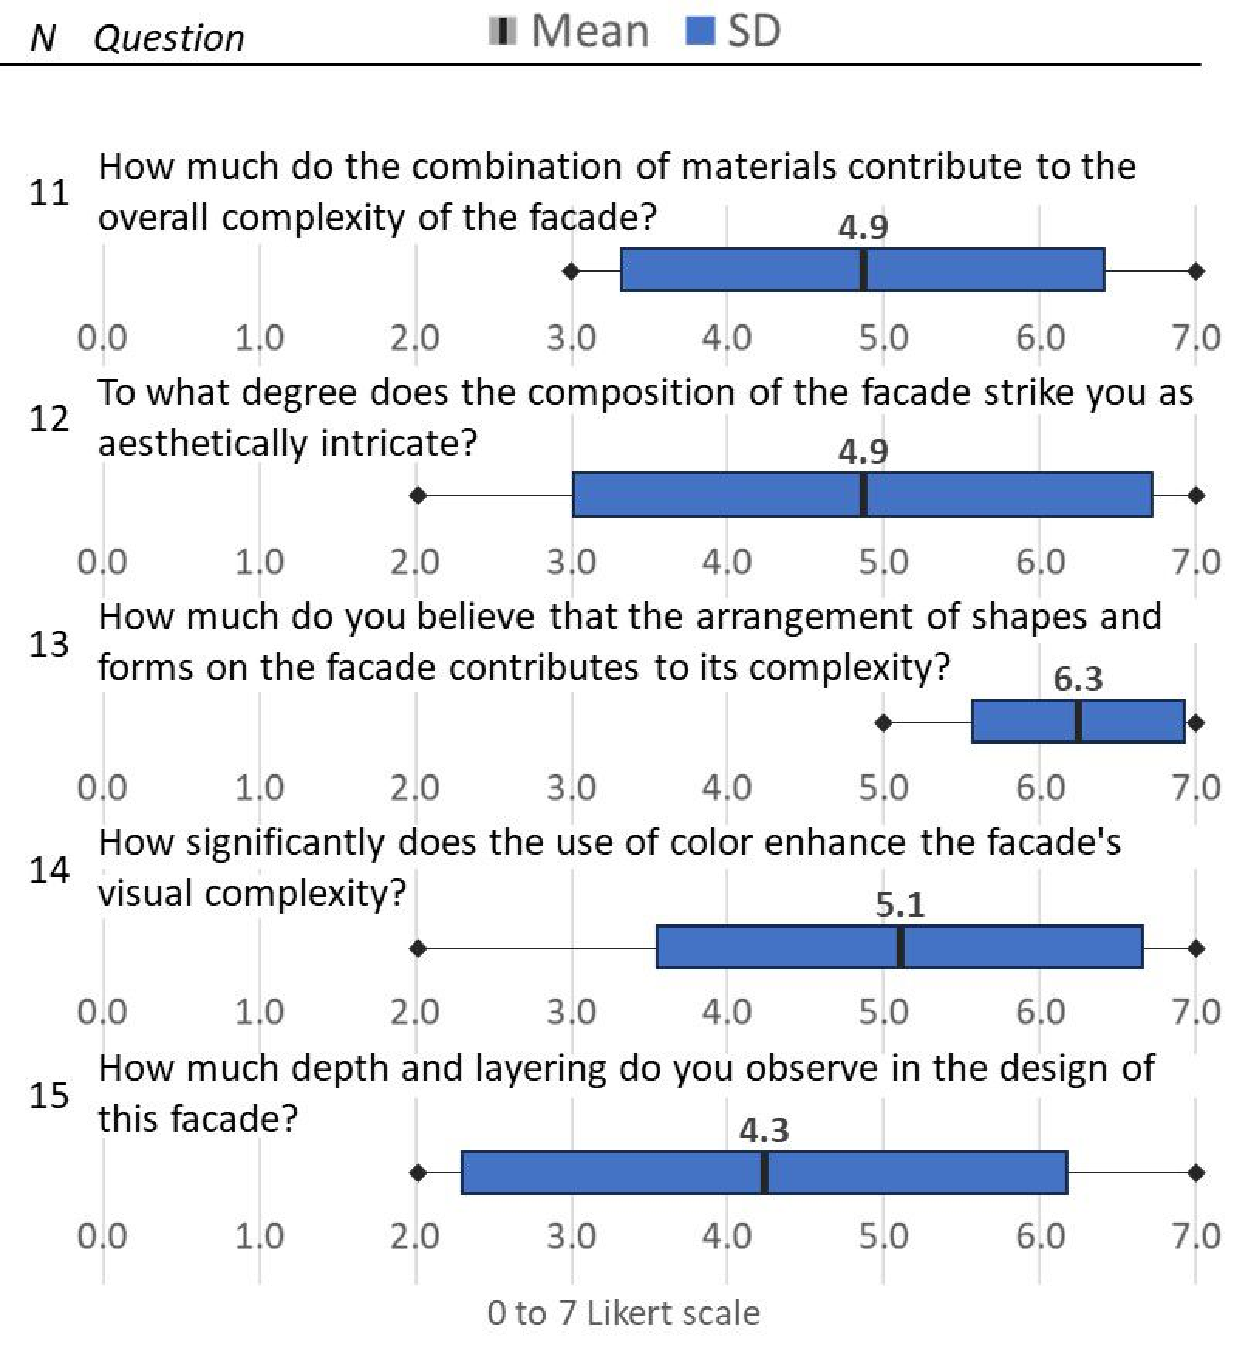
\includegraphics[width=\linewidth]{Images/SurveyPart2Complexity}
            \captionof{figure}{User-System Influence Perception section" questions. \- (n = 17), 1 - strongly disagree, 7 - strongly agree}
            \label{fig:SurveyQuestions11-15}
        \end{tabularx}
    \end{table*}


During post-experiment interviews, participants were asked for their opinions on the weight distribution used by the optimization model to balance the trade-offs between the three performance indicators.
The initial distribution decided for the system was set at 50, 30, and 20 for the respective indicators (see Table \ref{tab:PerformanceIndicators}).
While most participants maintained a consistent criteria for ranking the indicators, slight deviations from the predetermined weight distribution were observed.
Figure \ref{fig:PerformanceIndicatorweightChart} visually represents the average weight configuration suggested by the participants, demonstrating their individual preferences in adjusting the trade-off weights for each site.

Overall, the results support the initial hypothesis, indicating that VR has the potential to enhance the acceptance of data-driven design recommendations in SLP. However, the "user satisfaction" section of the survey, summarized in Figure \ref{fig:UsabilityChartSurvey}, revealed room for improvement in the user interface and experience, with scores above 4.5 on a 7-point Likert scale.
Notably, the areas of helpfulness and visualization enhancement ranked the lowest, despite initially being considered key advantages of the "VR interaction" system compared to the "screen-based" alternative.
